\sectioncounter{12}
  \section{导数的意义}
  
  \subsection{知识梳理}
  由导数定义的来源可知, 利用导数可以求出物体运动的瞬时速率 (物理意义), 
  也可以求出函数图象上一点切线的斜率 (几何意义). 
  下面分别举例说明如何求瞬时速率函数和切线的方程.
  
  先考虑瞬时速率. 若一物体运动的路程 $s$ (单位: m) 与时刻 $t$ (单位: s) 满足 $s=s(t)=t^2 +3t$, 则瞬时速率函数 $v(t)= s'(t)= 2t+3$, 
  而 $t=1$ (s) 时, 物体的瞬时速率为 $v(1)=5$ m/s.
  
  再考虑切线的斜率. 设曲线 $C\colon y=f(x)=x^3$, 
  则 $C$ 上横坐标为 $x$ 的点处切线的斜率 $k=f'(x)=3x^2$.
  点 $(1,1)$ 在 $C$ 上, 该点处 $C$ 的切线斜率为 $f'(1)= 3$.
  由直线的点斜式方程, 对应的切线方程为 
  \[y-1=3(x-1), \text{\ 即\ }y=3x-2.\]
  
  把后一个例子一般化: 设曲线 $C\colon y=f(x)$, 
  则 $C$ 上点 $x_0$ 处切线的斜率 $k=f'(x_0)$, 而切线的方程为 
  \[y-f(x_0)= f'(x_0)(x-x_0).\]
  结论表明, 函数的解析式和切点的横坐标决定了切线的方程.

  \lianxi
  \begin{exercise}
    求曲线 $y=2x^2 +1$ 在点 $P(-1,3)$ 处的切线方程.
  \end{exercise}

  \beginsolution
    $y'=4x$, 切线斜率 $k=-4$, 方程为 $y=-4x-1$.
  \endsolution
  
  \begin{exercise}
    求函数 $f(x)=\dfrac1{\sqrt{x}}$ 的图象在点~$(1,1)$ 处的切线方程.
  \end{exercise}

  \beginsolution
    $f'(x)=-\frac12x^{-\frac32}$, 切线斜率 $k=-\frac12$, 方程为 $y=-\frac12x+\frac12$.
  \endsolution
    
  \begin{exercise}
    火箭升空后的一段时间内, $t$\,s 时的高度 $h(t)=5t^3 +30t^2 +45t+4$ (m), 
    则火箭的速度何时达到 120\,m/s\,?
  \end{exercise}

  \beginsolution
    $h'(t)=15t^2+60t+45=120$, 解得 $t=-5$ (舍) 或 $1$.
  \endsolution
  
  \subsection{要点导学\quad 各个击破}

  \subsubsection{切线的方程}
  \begin{example}
    已知函数 $f(x)=-\ln x -ax^2 +x$ ($a>0$). 若 $f'(1)=f'(2)$, 
    求 $f(x)$ 的图象在点 $(1,f(1))$ 处的切线方程.
  \end{example}

  \beginsolution
    $f'(x)=-\frac1x-2ax+1$. 由 $f'(1)=f'(2)$ 解得 $a=\frac14$, 则
    \[f(x)=-\ln x-\frac{x^2}4+x,\quad f'(x)=-\frac1x-\frac{x}2+1,\]
    即切点 $\Big(1,\frac34\Big)$, 切线斜率为 $f'(1)=-\frac12$, 方程为 $y=-\frac12x+\frac54$.
  \endsolution
  
  \begin{example}
    若曲线 $y=ax^2 +\dfrac{b}x$ ($a$, $b$ 为常数) 过点 $P(2,-5)$, 
    且在该点处的切线与直线 $7x+2y+3=0$ 平行, 求 $a+b$ 的值.
  \end{example}

  \beginsolution
    $y'=2ax-\frac{b}{x^2}$, 则
    \[\left\{\!\!\begin{array}{l}
        4a+\frac{b}2=-5,\\[5pt]
        4a-\frac{b}4=-\frac72,\end{array}\right.\quad
        \text{解得}
      \left\{\!\!\begin{array}{l}
        a=-1,\\
        b=-2,\end{array}\right.\]
    故 $a+b=-3$.
  \endsolution
  
  \lianxi
  \begin{exercise}
    若曲线 $y=\mathrm{e}^x$ 上点 $P$ 处的切线垂直于直线 $2x+y+1=0$, 
    求点 $P$ 的坐标.
  \end{exercise}

  \beginsolution
    $y'=\mathrm{e}^x=\frac12$, 解得 $x=-\ln2$, 则 $P\Bigl(-\ln2,\frac12\Bigr)$.
    
    \varexercise 曲线 $y=\mathrm{e}^x$ 上是否存在两点, 使得两点处的切线互相垂直?
    
    假设符合题意的两点存在, 设为 $A(a,\mathrm{e}^a)$, $B(b,\mathrm{e}^b)$. 由 $y'=\mathrm{e}^x$ 知 $\mathrm{e}^a\cdot\mathrm{e}^b=-1$, 不可能, 故符合题意的两点不存在.
  \endsolution
  
  \begin{exercise}
    若曲线 $y=x^2$ 的一条切线的斜率是 $-4$, 求该切线的方程.
  \end{exercise}

  \beginsolution
    $y'=2x=-4$, 解得 $x=-2$, 切点 $(-2,4)$, 切线方程为 $y=-4x-4$.
    
    \varexercise 曲线 $y=x^2$ 上是否存在两点, 使得两点处的切线互相垂直?
        
    假设符合题意的两点存在, 设为 $A(a,a^2)$, $B(b,b^2)$. 由 $y'=2x$ 知 $2a\cdot2b=-1$, 即 $ab=-\frac14$, 故符合题意的两点存在.
    
    \varexercise 若曲线 $y=x^2$ 上两点 $A$, $B$ 处的切线互相垂直且交于点 $P$, 求证: 点 $P$ 在定直线上.
    
    设 $A(a,a^2)$, $B(b,b^2)$, 已有 $ab=-\frac14$. 而
    \mymarginpar{直线 $y=-\frac14$ 恰为抛物线 $y=x^2$ 的准线. 逆命题: ``过抛物线 $C$ 的准线 $l$ 上任一点作 $C$ 的两切线 $l_1$, $l_2$, 则 $l_1\perp l_2$.'' 也成立 (如何证明?).}
    \[PA\colon y-a^2=2a(x-a),\quad PB\colon y-b^2=2b(x-b),\]
    联立解得 $P\Bigl(\frac{a+b}2,ab\Bigr)$, 即点 $P$ 在定直线 $y=-\frac14$ 上.
  \endsolution
  
  \subsubsection{切线方程的应用}
  \begin{example}
    若曲线 $f(x)=x^{-2}$ 在点 $(a,a^{-2})$ ($a>0$) 处的切线与两条坐标轴围成的三角形的面积为 $3$, 求 $\log_{\frac{\sqrt3}2} a$ 的值.
  \end{example}

  \beginsolution
    $f'(x)=-2x^{-3}$, 则点 $(a,a^{-2})$ 处的切线方程为 $y=-2a^{-3}x+3a^{-2}$, 与 $x$ 轴交于点 $\Big(\frac{3a}2,0\Big)$, 与 $y$ 轴交于点 $\Big(0,\frac3{a^2}\Big)$, 所以 
    \[3=\frac12\cdot \frac{3a}2\cdot \frac3{a^2},\quad a=\frac34,\]
    因此 $\log_{\frac{\sqrt3}2} a=2$.
  \endsolution
  
  \lianxi
  \begin{exercise}
    若 $y=x^a +1$ ($a\in\mathbb{R}$) 在点 $(1,2)$ 处的切线经过坐标原点,
    求 $a$ 的值.
  \end{exercise}

  \beginsolution
    $y'=ax^{a-1}$. 方法一: 在点 $(1,2)$ 处的切线为 $y-2=a(x-1)$, 则 $-2=a\cdot(-1)$, $a=2$.
    \mymarginpar{切线斜率既可由导数算出, 也可由切线上两点坐标算出.}
    
    方法二: 在点 $(1,2)$ 处的切线为 $y=2x$, 则 $a\cdot 1^{a-1}=2$, $a=2$.
  \endsolution
  
  \begin{exercise}
    已知直线 $f(x)=kx+1$ 与曲线 $g(x)=x^3 +ax+b$ 切于点 $(1,3)$, 
    求实数 $b$ 的值.
  \end{exercise}

  \beginsolution
    $f'(x)=k$, $g'(x)=3x^2+a$, 则
    \mymarginpar{公切点处有公切线, 一般转化为切点处纵坐标和切线斜率均相等.}
    \[\left\{\!\!\begin{array}{l}
      k= 3\cdot 1^2+a,\\
      k+1=1+a+b=3,
      \end{array}\right.\]
    解得 $a=-1$, $b=3$, $k=2$.
  \endsolution
  
  \subsubsection{课堂评价}
  \begin{exercise}
    设函数 $f(x)=ax+\dfrac{b}x$ ($a$, $b\in\mathbb{R}$), 
    若 $f(x)$ 在点 $(1,f(1))$ 处的切线斜率为 $1$, 求 $a$ 与 $b$ 的等量关系.
  \end{exercise}

  \beginsolution
    $f'(x)=a-\frac{b}{x^2}$, 而 $f'(1)=1$, 则 $a-b=1$.
  \endsolution
  
  \begin{exercise}
    设曲线 $y=ax-\ln(x+1)$ 在点 $(0,0)$ 处的切线方程为 $y=2x$, 求 $a$ 的值.
  \end{exercise}

  \beginsolution
    $y'=a-\frac1{x+1}$, 令 $x=0$, 则 $a-1=2$, $a=3$.
  \endsolution
  
  \begin{exercise}
    若曲线 $y=ax^2 -\ln x$ 在点 $(1,a)$ 处的切线平行于 $x$ 轴, 求 $a$ 的值.
  \end{exercise}

  \beginsolution
    $y'=2ax-\frac1x$, 令 $x=1$, 则 $2a-1=0$, $a=\frac12$.
  \endsolution
  
  \begin{exercise}
    已知函数 $f(x)=ax^2 -\dfrac12 x+2\ln(x+1)$, 求其图象在点 $(0,f(0))$ 处的切线方程.
  \end{exercise}

  \beginsolution
    $f'(x)=2ax-\frac12+\frac2{x+1}$, 则 $f'(0)=\frac32$, 而 $f(0)=0$, 故所求切线方程为 $y=\frac32 x$.
  \endsolution
  
  \subsection{课后练习}
  \begin{exercise}
    求曲线 $y=x\mathrm{e}^x$ 在点 $(1,\mathrm{e})$ 处的切线斜率.
  \end{exercise}

  \beginsolution
    $y'=(x+1)\mathrm{e}^x$, 令 $x=1$, 则 $y'=2\mathrm{e}$.
  \endsolution
  
  \begin{exercise}
    求曲线 $y=-5\mathrm{e}^x +3$ 在点 $(0,-2)$ 处的切线方程.
  \end{exercise}

  \beginsolution
    $y'=-5\mathrm{e}^x$, 令 $x=0$, 则 $y'=-5$, 切线方程为 $y=-5x-2$.
  \endsolution
  
  \begin{exercise}
    如图~\ref{fig-190419-2140}, 曲线 $y=f(x)$ 在点 $P$ 处的切线方程是 $y=-x+8$, 求 $f(5)+f'(5)$ 的值.
    \begin{figure}[htb]
    \small
    \centering
    \begin{minipage}[b]{0.4\linewidth}
    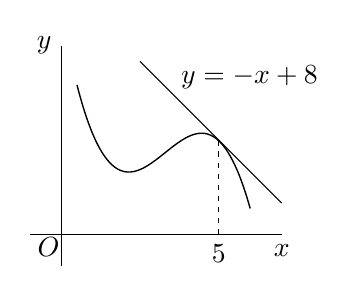
\begin{tikzpicture}[scale=0.4]
      \draw[\myaxisarrow] (-1,0) -- (7,0) node[below] {$x$};
      \draw[\myaxisarrow] (0,-1) -- (0,6) node[left] {$y$};
      \draw[line width=0.5pt,smooth,samples=100,domain=0.5:6] 
        plot(\x,{2.6-(\x-3.3)^3/5+4*(\x-3.3)/5});
      \draw (2.5,5.5)--(7,1);
      \draw[line width=0.5pt,dash pattern= on 2pt off 2pt] (5,0)--(5,3);
      \draw (3.5,5) node[right] {$y=-x+8$};
      \draw (5,0) node[below] {$5$};
      \draw (-0.4,-0.4) node {$O$};
    \end{tikzpicture}
    \caption{}\label{fig-190419-2140}
    \end{minipage}
    \hskip 1cm%
    \begin{minipage}[b]{0.4\linewidth}
    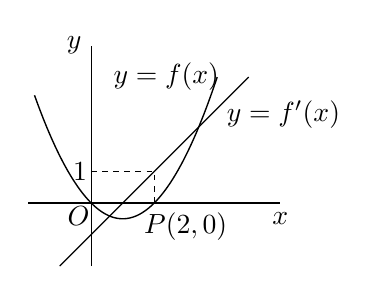
\begin{tikzpicture}[scale=0.4]
      \draw[\myaxisarrow] (-2,0) -- (6,0) node[below] {$x$};
      \draw[\myaxisarrow] (0,-2) -- (0,5) node[left] {$y$};
      \draw[line width=0.5pt,smooth,samples=100,domain=-1.8:4] 
        plot(\x,{(\x)^2/2-\x});
      \draw (-1,-2)--(5,4);
      \draw[line width=0.5pt,dash pattern= on 2pt off 2pt] (0,1)--(2,1)--(2,0);
      \draw (3,0) node[below] {$P(2,0)$};
      \draw (0,1) node[left,xshift=2pt] {$1$};
      \draw (0.4,4) node[right] {$y=f(x)$};
      \draw (4,2.8) node[right] {$y=f'(x)$};
      \draw (-0.4,-0.4) node {$O$};
    \end{tikzpicture}
    \caption{}\label{fig-190419-2150}
    \end{minipage}
    \end{figure}
  \end{exercise}

  \beginsolution
    由图, $f(5)=3$, $f'(5)=-1$, 则 $f(5)+f'(5)=2$.
  \endsolution
  
  \begin{exercise}
    已知函数 $y=f(x)$ 及其导函数 $y=f'(x)$ 的图象如图~\ref{fig-190419-2150} 所示, 求曲线 $y=f(x)$ 在点 $P$ 处的切线方程.
  \end{exercise}

  \beginsolution
    由 $P(2,0)$ 知 $f'(2)=1$, 则切线方程为 $y=x-2$.
  \endsolution
  
  \begin{exercise}
    求曲线 $y=\dfrac{\mathrm{e}^x}x$ 在点 $\Big(2, \dfrac{\mathrm{e}^2}2\Big)$ 
    处的切线方程.
  \end{exercise}

  \beginsolution
    $y'=\frac{(x-1)\mathrm{e}^x}{x^2}$, 令 $x=2$, 则 $y'=\frac{\mathrm{e}^2}4$, 所求的切线方程为 $y=\frac{\mathrm{e}^2}4 x$.
  \endsolution

  \begin{exercise}
    若直线 $l$ 是曲线 $y= \dfrac13 x^3 +x$ 的切线且倾斜角最小, 求 $l$ 的方程.
  \end{exercise}

  \beginsolution
    $y'=x^2+1\geqslant 1$, 故倾斜角取值范围为 $\Bigl[\frac{\pi}4,\pi\Bigr)$, 表明 $l$ 的倾斜角为 $\frac\pi4$, 斜率为 $1$, 切点为 $(0,0)$, $l$ 的方程为 $y=x$.
  \endsolution
  
  \begin{exercise}
    已知函数 $f(x)=x^3 -3x^2 +ax+2$, 曲线 $y=f(x)$ 在点 $(0,2)$ 处的切线与 $x$ 轴交点的横坐标为 $-2$, 求 $a$ 的值.
  \end{exercise}

  \beginsolution
    $f'(x)=3x^2-6x+a$, $f'(0)=a$, 曲线在点 $(0,2)$ 处的切线方程为 $y=ax+2$. 把 $(-2,0)$ 代入, $-2a+2=0$, 则 $a=1$.
  \endsolution
  
  \begin{exercise}
    求曲线 $y=\dfrac13 x^3 +x$ 在点 $\Big(1,\frac43\Big)$ 处的切线与坐标轴所围成的三角形的面积.
  \end{exercise}
  

  \beginsolution
    $y'= x^2+1$, 令 $x=1$, 则 $y'=2$, 曲线在点 $\Big(1,\frac43\Big)$ 处的切线方程为 $y=2x-\frac23$, 与 $x$ 轴交于点 $\Big(\frac13,0\Big)$, 与 $y$ 轴交于点 $\Big(0,-\frac23\Big)$, 故所求三角形面积为 $\frac12\cdot \frac13\cdot \frac23= \frac19$.
  \endsolution

%%%%%%%%%%%%%%%%%%%%%%%%%%%%